\documentclass[11pt]{article}

\usepackage{wrapfig}
\usepackage{subfig}
\usepackage{graphicx}
\usepackage{hyperref}
\usepackage{amsmath}
\usepackage{a4wide}
\usepackage{multirow}
\usepackage{minted}

\def\thetitle{Advanced Vision 2011/2012\\ Practical 3}
\def\theauthor{Steven Skelton (s0824321) and Wenqi Yao (s0838969)}

% TITLE PAGE
\title{\thetitle}
\author{\theauthor}
\date{}

\begin{document}

\maketitle
\thispagestyle{empty}

\section{Introduction}

In this assignment, we were tasked with augmenting a sequence of images, via homographic transfer of a given background image, and a sequence of images from a separate video. We utilised various algorithms to build a system that can robustly extract the person from in front of the wall and transfer the given background; as well as locate the rectangular plane fairly reliably to transfer the video onto it. 

\section{Algorithms}
\subsection{Finding the Background}
The points in the trapezoid are found manually and hard-coded into the background-finding algorithm. 

To find the points of interest (within the back wall), the equations of the lines between neighbouring corners are found. Naive interpolation is used to find pixels on the lines. Each row of pixels within the bounding rectangle are scanned to find the left-most and right-most pixels in each line. All pixels between these two pixels (inclusive) are marked on a indicator matrix of size \emph{480 x 640}. 

To find the foreground, the z-values for each pixel are averaged over the first 7 frames (before the man walks in). In each frame, the foreground is then given by every pixel that is at least a threshold value in front of its mean value. At the top of the image, the pixels are further away and have a smaller variance. Many pixels remain as background pixels throughout, and hence many of them are cast as ``foreground" pixels over different frames (as seen in Figure \ref{fig:failbg2} ). Hence, the threshold value is set at 0.1. At the bottom of the image, the pixels are nearer, with a large variance. Most of the pixels will be covered by the walking man's legs in at least one frame. Using 0.1 as the threshold value hence causes incorrect classification of the man's trousers as the background (as seen in Figure \ref{fig:failbg} ). Instead, the threshold is set to the standard deviation of each pixel over all frames. 

The classified background pixels are then masked with the indicator matrix.

\begin{figure}
  \centering
  \subfloat[Threshold 1std]{\label{fig:failbg2}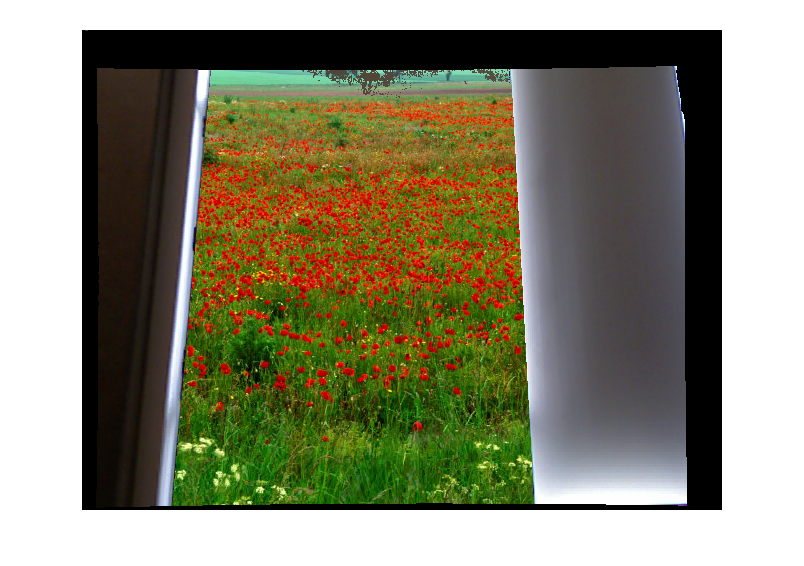
\includegraphics[width=0.5\textwidth]{missingbg}} ~
  \subfloat[Threshold 0.1]{\label{fig:failbg}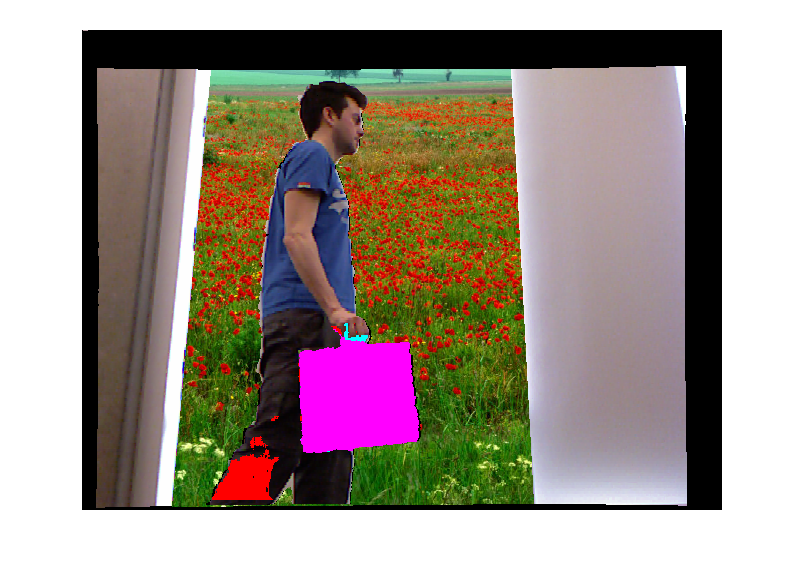
\includegraphics[width=0.5\textwidth]{floatingman}} 
  \caption{Setting the threshold to either 0.1 or 1 standard deviation above the mean results in errors. In \ref{fig:failbg2}, not all the pixels at the top of the image are coloured in. In \ref{fig:failbg} the man's legs float above the bottom line of grass. The red and magenta colouring are a due to foreground detection. To solve this, a mixture of these two was used.}
  \label{fig:failing}
\end{figure}

\subsection{Image Transfer}

To transfer the given image of the field onto the background pixels, the given code for homographic transfer \emph{(esthomog.m)} is used. Due to the crude nature of the interpolation between corners, some of the pixels in the background area map to points just outside the boundaries of the field image. These pixels are capped to the boundary of the field image. The results of this can be seen in Figure \ref{fig:proj}.

\begin{figure}[h]
  \centering
  \subfloat{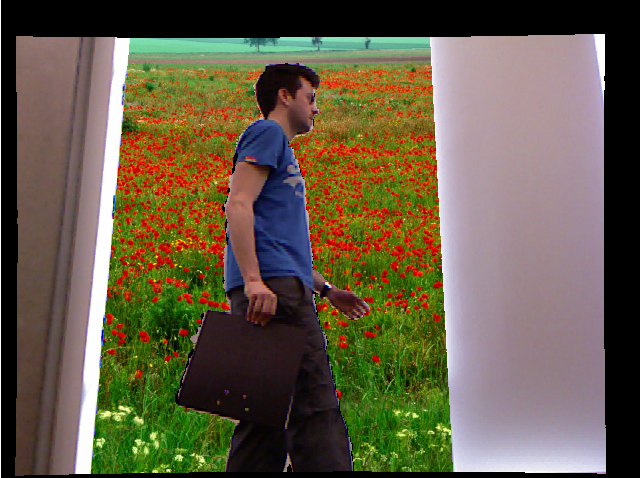
\includegraphics[width=0.35\textwidth]{proj1}} ~
  \subfloat{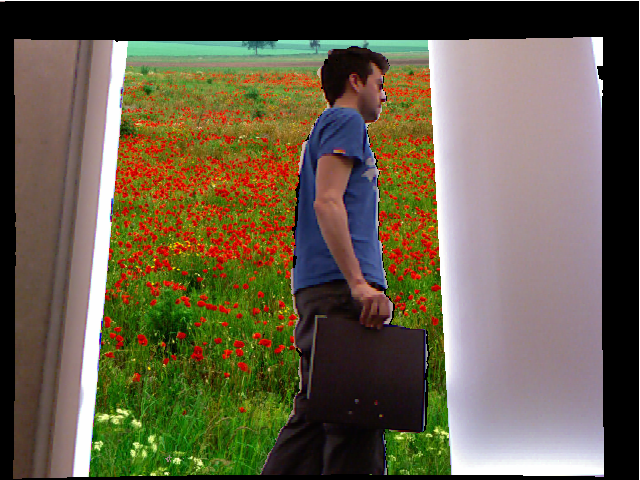
\includegraphics[width=0.35\textwidth]{proj3}} 
  \hspace{0pt}
  \subfloat{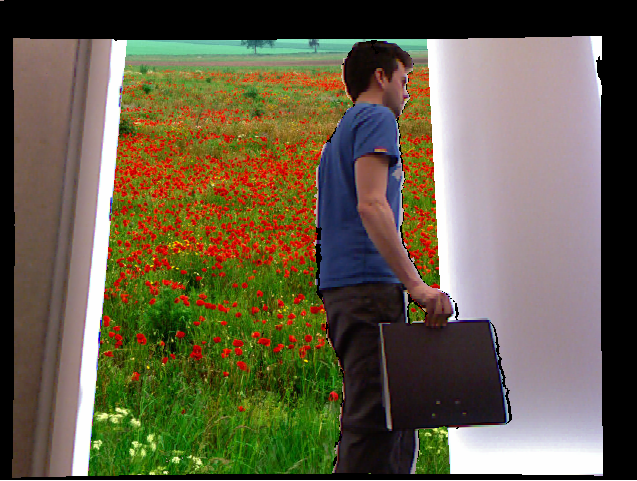
\includegraphics[width=0.35\textwidth]{proj4}} ~
  \subfloat{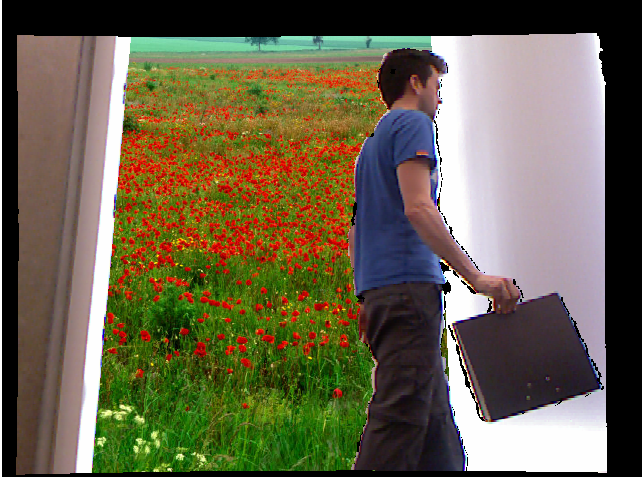
\includegraphics[width=0.35\textwidth]{proj5}}
  \caption{Frames after transferring the background image.}
  \label{fig:proj}
\end{figure}

\subsection{Finding the Rectangular Plane}

Various techniques were used in attempts to find the rectangular plane. 

\subsubsection{Pruning the Search Space}
The search space was first pruned to find the foreground pixels, as the rectangular plane can only lie in the foreground (estimated at the mean of the z-values for that frame + 0.36), and in the bottom half of the image. The results of this can be found in Figure \ref{fig:notbg}.

\begin{figure}
  \centering
  \subfloat{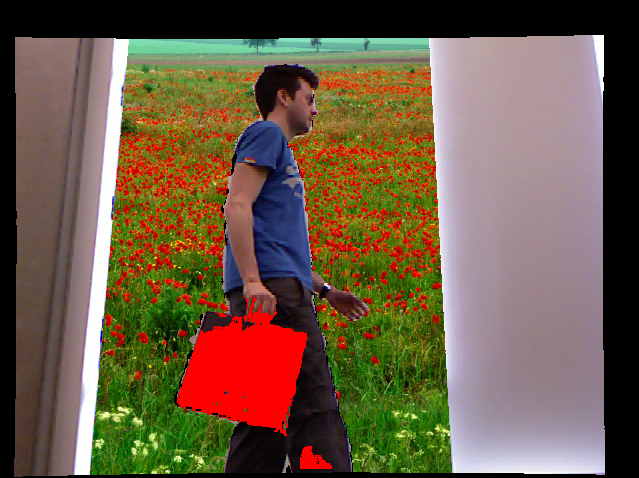
\includegraphics[width=0.35\textwidth]{notbg1}} ~
  \subfloat{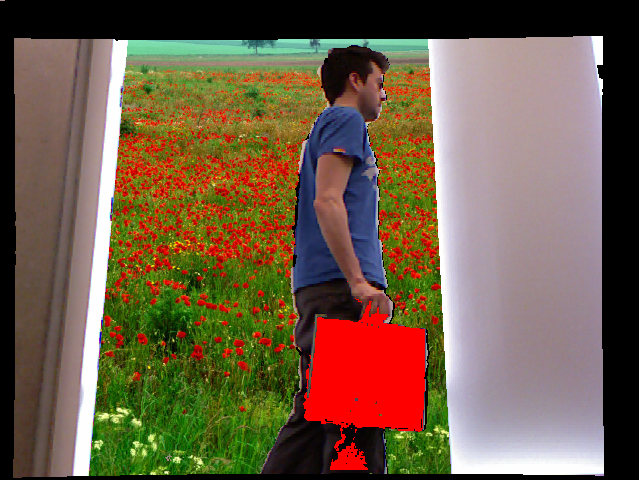
\includegraphics[width=0.35\textwidth]{notbg3}} \\
  \subfloat{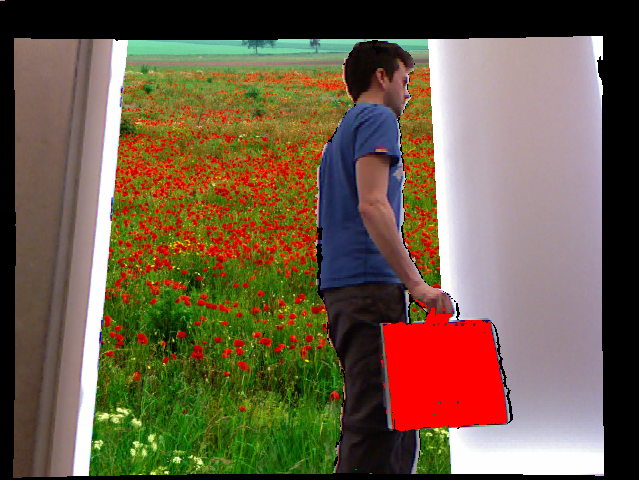
\includegraphics[width=0.35\textwidth]{notbg4}} ~
  \subfloat{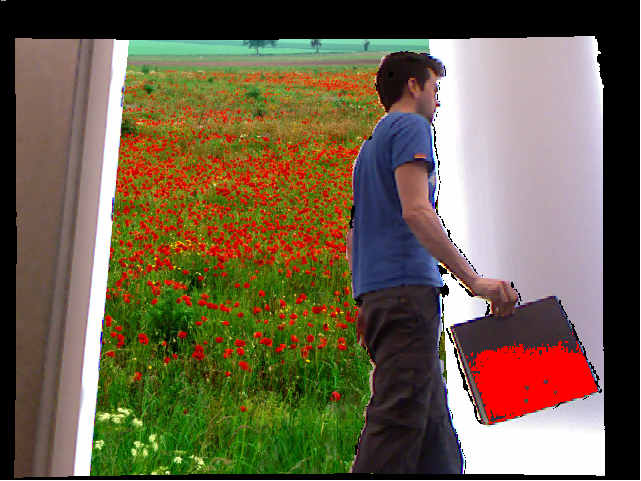
\includegraphics[width=0.35\textwidth]{notbg5}}
  \caption{Frames after finding the foreground pixels that match the correct colour. Some of the hand and leg pixels are included, and some of the rectangular pixels are missing.}
  \label{fig:notbg}
\end{figure}

\subsubsection{RANSAC}
A RANSAC plane-finding algorithm was tried. In each iteration, 3 random points were picked and a plane was fit to them. If the number of points within the search space that fit the plane (to a given threshold, around 0.005) was between 10000 and 15000, the plane was considered as a candidate plane. After 100 iterations, the candidate plane with the smallest sum error between itself and the points that lay on it was returned. 

The problem with this method was that it was extremely slow, and often returned planes that did not contain all of the points contained in the rectangular plane. As such, it was rejected in favour of simpler methods.

\subsubsection{Plane Fitting}
Instead of randomly fitting planes to 3 points within the search space, a plane was fit to all the points of the largest connected components of the current search space (using \emph{fitplane.m}). As the pruned search space may not contain all of the pixels on the plane, the plane is fit to all of the pixels in the lower half of the image. The results of this can be seen in Figure \ref{fig:plane}.

\begin{figure}
  \centering
  \subfloat{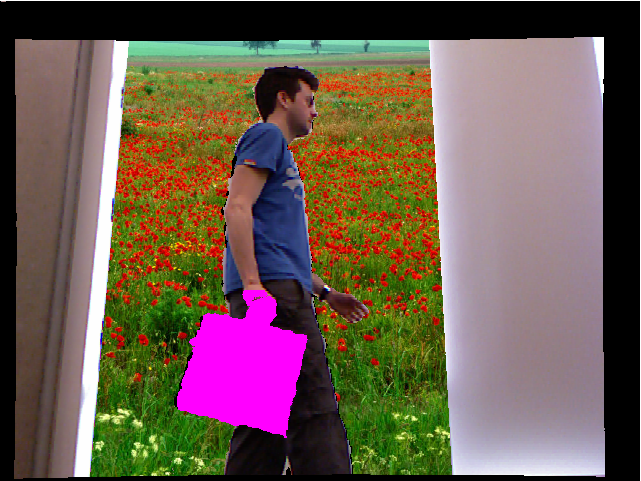
\includegraphics[width=0.35\textwidth]{plane1}} ~
  \subfloat{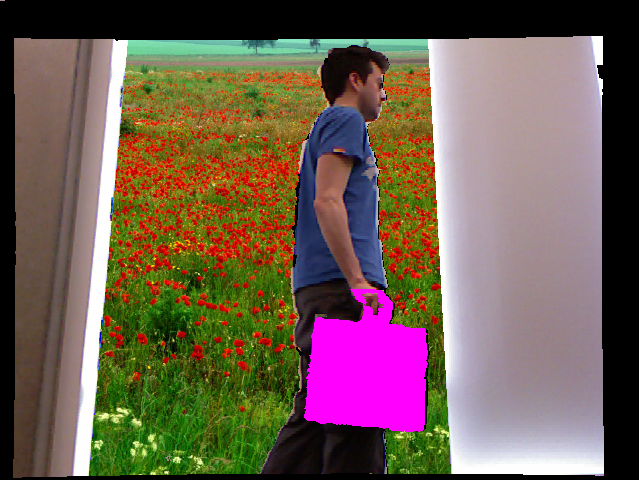
\includegraphics[width=0.35\textwidth]{plane3}} \\
  \subfloat{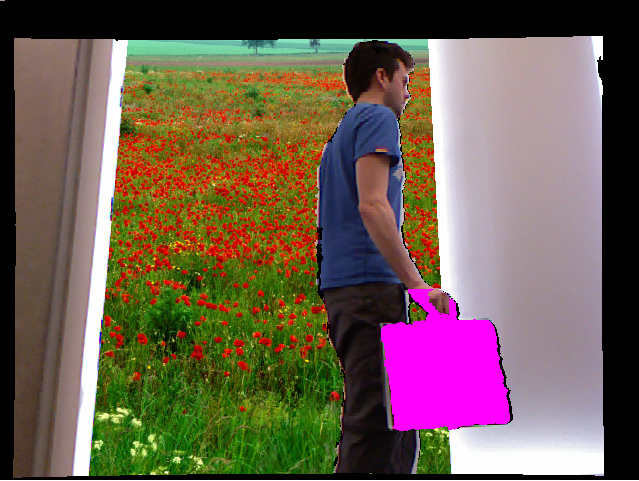
\includegraphics[width=0.35\textwidth]{plane4}} ~
  \subfloat{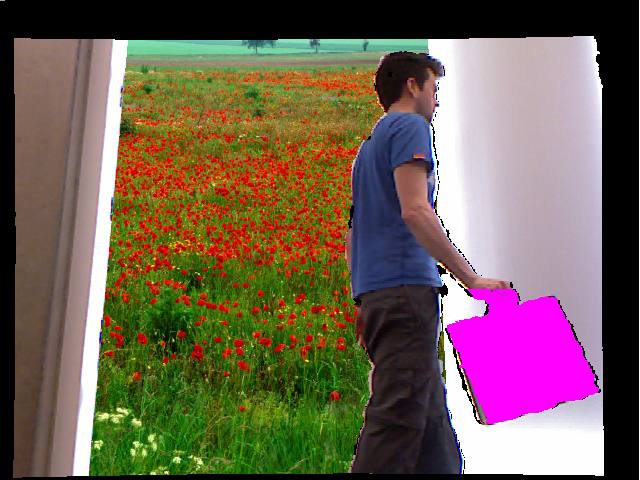
\includegraphics[width=0.35\textwidth]{plane5}}
  \caption{Largest connected component of the plane fit to the data. The leg pixels have been removed, and all of the rectangular plane is covered. However, more of the hand pixels are also in the plane.}
  \label{fig:plane}
\end{figure}

\subsection{Video Transfer}

\begin{wrapfigure}{r}{0.4\textwidth}
  \vspace{-20pt}
  \begin{center}
    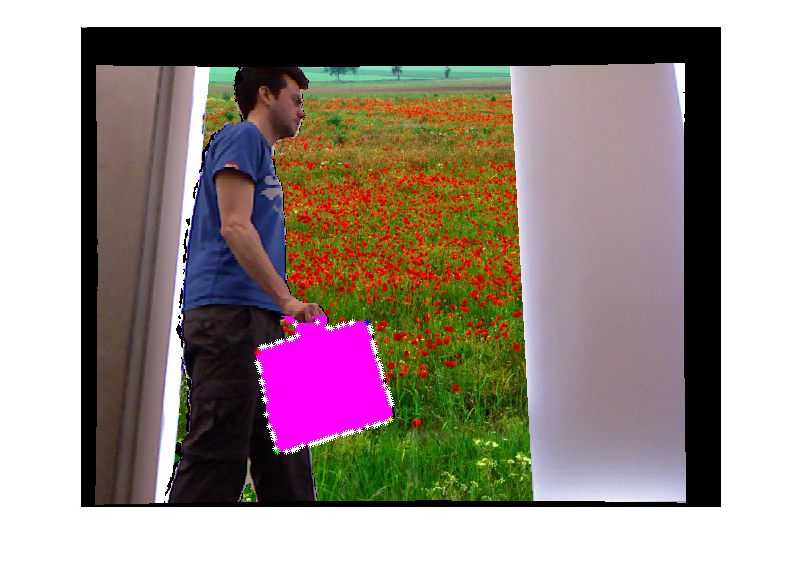
\includegraphics[width=0.38\textwidth]{corners}
  \end{center}
  \vspace{-20pt}
  \caption{Corner points of the plane that were found. The RGBY asterisks represent the corners selected by the system.}
  \vspace{-20pt}
\end{wrapfigure}

Homographic transfer required the 4 corner points of the rectangle. To find this, the binary image of the rectangle was opened using a rectangular structuring element to emphasise the corners. Matlab's \emph{corner} function was then performed on the binary image. This produced many unnecessary corners, caused by the jagged edges of the binary image. As the largest connected component of the plane often included parts of the hand, these corners were filtered to ensure that they were not too high. The threshold was set at 130px higher than the lowest corner found. The four corners were selected as the two pairs of points with the largest distance between them. To protect against noise,  the corners selected had to be at least 50 pixels apart. 

Transfer of the moving image was done similarly to that of the background image. As the plane rotated (such that the top-most point could either be in the left or right corner), the points had to be sorted both by x and y-coordinates, and then ordered clockwise.

\section{Results}

\begin{figure}[h]
  \centering
  \subfloat{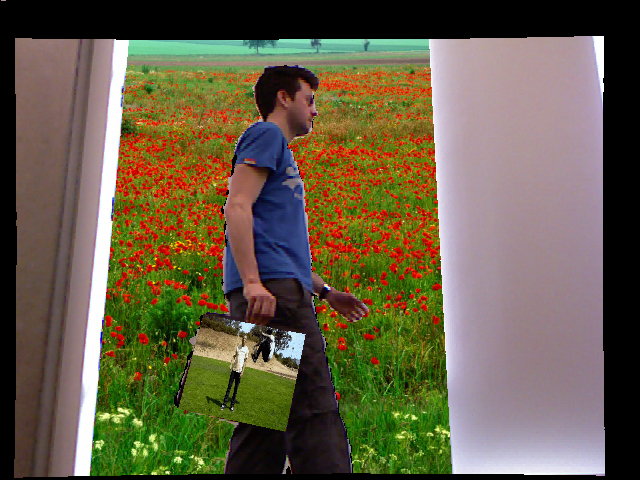
\includegraphics[width=0.35\textwidth]{d1}} ~
  \subfloat{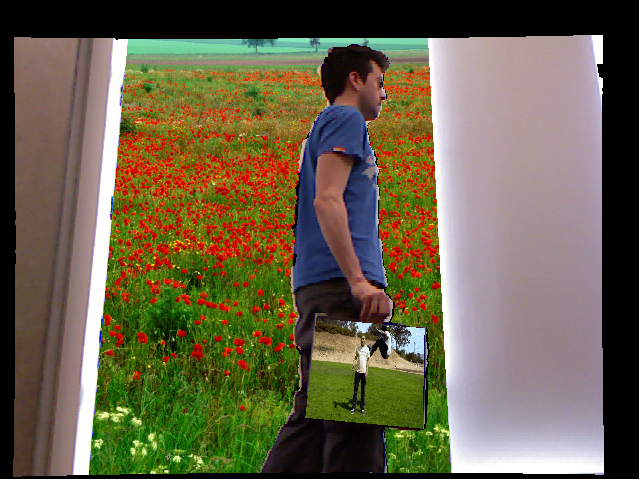
\includegraphics[width=0.35\textwidth]{d3}} \\
  \subfloat{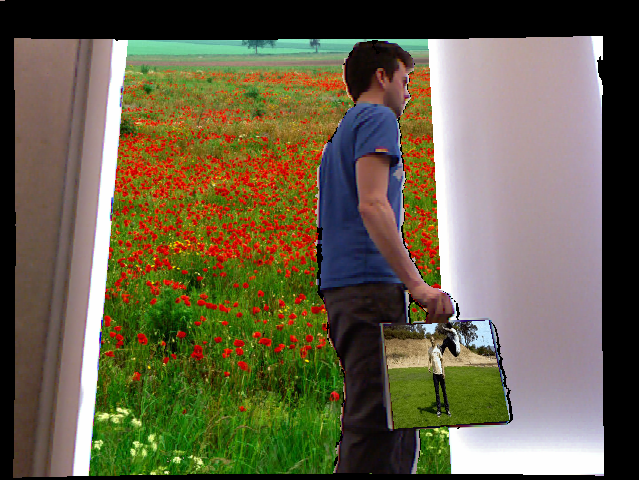
\includegraphics[width=0.35\textwidth]{d4}} ~
  \subfloat{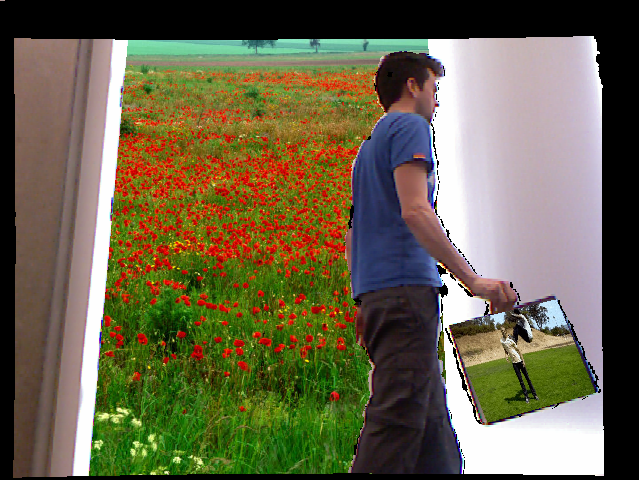
\includegraphics[width=0.35\textwidth]{d5}}
  \caption{Final results.}
  \label{fig:final}
\end{figure}

Our system performed perfectly in finding the background and transferring the background image for all 36 frames. This was likely due to the robust thresholding system. It also managed to find the rectangular plane and transfer the image on 32 out of 36 frames. Final results can are as in Figure \ref{fig:final}. The frames that failed, as well as explanations for failure are given below: 

\begin{figure}[h]
  \centering
  \subfloat[Frame 14]{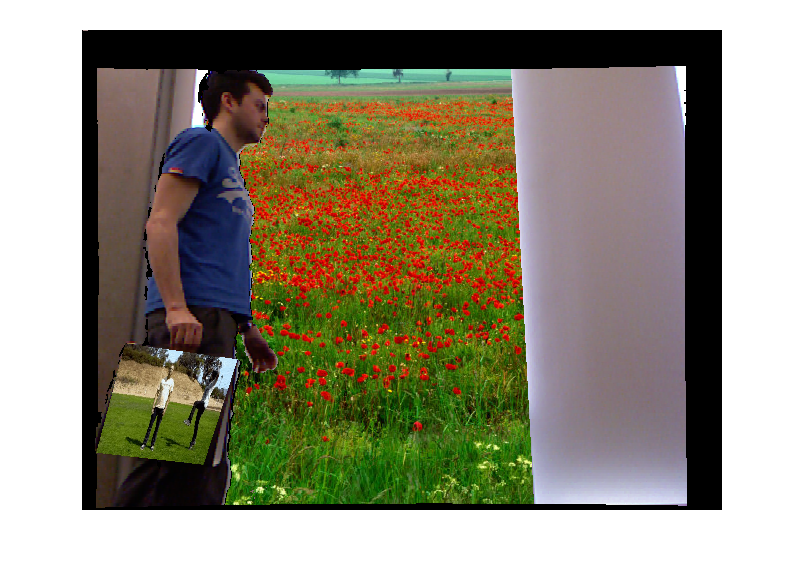
\includegraphics[width=0.24\textwidth]{fail0}} ~
  \subfloat[Frame 15]{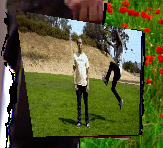
\includegraphics[width=0.24\textwidth]{fail1}} ~
  \subfloat[Frame 19]{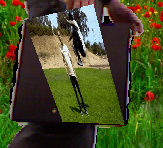
\includegraphics[width=0.24\textwidth]{fail2}} ~
  \subfloat[Frame 26]{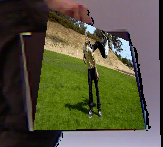
\includegraphics[width=0.24\textwidth]{fail3}} ~
  \caption{Frames that failed to transfer the video images well. Most of these were due to problems with the fit of the plane.}
  \label{fig:failvid}
\end{figure}

Plane-fitting was a large limitation - The rectangular plane was not always fully flat, causing several problems. In Frame 14, various points on the bottom-right of the actual plane did not fit to the calculated plane. As such, the corner-finding algorithm failed to find the actual corner. In Frame 15, creasing on the man's trousers caused pixels on them to fit to the plane. Since they were still relatively close to the rest of the plane, these pixels were not filtered out. In Frame 19, the calculated plane was a very poor fit to the actual plane, and only fit a diagonal strip from top left to bottom right. Hence it was impossible for the corner detection to pick out the correct points. In Frame 26, the correct plane was detected with the plane-fitting algorithm. However, parts of the man's hand also fit the plane, and the furthest distance between points was found incorrectly. 

These results suggest that improvements should be made to the fitting of the plane. It might be beneficial to filter on the colour and z-value of the pixels after fitting the plane. Rudimentary versions of this were attempted, by only accepting darker colours (with a low RGB sum) and values smaller than a threshold value from the maximum (closest) z-value. This managed to remove a few incorrectly classified pixels, but were not helpful to the overall result. Better filter conditions are required to improve this. With a better filter, the threshold for the plane fit can then be relaxed, allowing the fit of all the points in the actual rectangular plane. Furthermore, improvements to the corner-picking algorithm could be used to prevent selection of pixels on the man's hand.

\section{Conclusion}
We have produced a system that reliably identifies background pixels and transfers a given image onto them, and finds and transfers a given video sequence onto a rectangular plane with reasonable accuracy. Areas for improvement include a more precise fit to the rectangular plane (perhaps back to a modified RANSAC method), as well as finding other features that separate the hand from the rectangular surface.

\appendix

\newpage

\section{Code Listing}

\subsection{run.m}

\begin{minted}{matlab}
%% run
% This file contains the main method for running the sequence of images and
% homography

%% Toggles
% Toggle mouse input to find new coordinates
find_new_points = 0; 

% Toggle write to video
write_video = 0;

%% Set up Homography
% Read the given background image
files = dir(fullfile('Images', '*.mat'));
field = imread('Images/field.jpg');

% Find the coordinates of the corners of the background image
[field_y, field_x,~] = size(field);
XY = [[1,1]',[1,field_x]',[field_y,1]',[field_y,field_x]']';

% Find the coordinates of the background plane
rect  = [ 41, 130; 477, 91; 474, 452; 40, 429 ];
UV = [[41, 130]', [40, 429]', [478, 91]', [477, 452]']'; 

% Read the images from the video being transferred
base = 'Images/kick/';
animation = cell(15,1);
for i = 1 : 15,
    animation{i} = imread(strcat(base,int2str(i),'.jpg'));
end

% Find the coordinates of the corners of the video to transfer
[anim_y, anim_x, ~] = size(animation{1});
XY_A  = [[1,1]',[1,anim_x]', [anim_y,1]', [anim_y,anim_x]']';  

%% Find the background plane and homographic transfer
bg_trapezoid = find_trapezoid(480, 640, rect);

P = esthomog(UV,XY,4);

n_files = length(files);
images = cell(1, n_files);
avg_z  = zeros(480, 640, n_files);

%% Set up video writer
if (write_video),
    vw = VideoWriter('AV_movie.avi');
    vw.FrameRate = 6;
    vw.open();
end

%% Preload images

for i = 1 : n_files,

    curr_image = load(fullfile('Images',files(i).name));    
    vars = fieldnames(curr_image);
    
    for j = 1:length(vars)
        assignin('base', vars{j}, curr_image.(vars{j}));
    end

    % Reshape from long array to 640x480x6 matrix    
    im = reshape(curr_image.(vars{1}), 640, 480, 6);
    
    % Swap dimensions 1 and 2
    final = permute(im, [2 1 3]);
    
    images{i} = final;
    avg_z(:,:,i) = final(:,:,3);
    
    % Configure the trapezoid, if necessary
    if (i == 1 && find_new_points),
        [X,Y] = ginput(4);
        for k = 1 : 4,
            disp(['Point ' num2str(k) ' is at (' num2str(X(k)) ',' ...
                num2str(Y(k)) ').']);
        end
    end
end

clear 'xyzrgb_*';
clear UV; clear XY;

%% Use the average z coordinates of the first 7 frames to find the wall
% The threshold for foreground images is 0.1 above the mean for the top
% half of the image, and one standard deviation above the mean, for the
% bottom half of the image.

new_avg_z = avg_z(:,:,1:7);
mean_z = mean(new_avg_z, 3);
variance_z = (avg_z - repmat(mean_z, [1,1,n_files])).^2;
std_z  = mean(variance_z, 3);
std_z(1:240,:) = 0.1;
threshold = mean_z + std_z;

%% Preload homography of background image

[I, J] = find(bg_trapezoid);

bg_projection = zeros(480, 680, 3);
for i = 1 : length(I),
   % Project destination pixel into source
   v = P * [ I(i), J(i), 1 ]';        
   % Undo projective scaling and round to nearest integer
   y = round(v(1)/v(3));              
   x = round(v(2)/v(3));
   if y == 0, y = 1; end
   if x == 0, x = 1; end
   if y > field_y, y = field_y; end
   if x > field_x, x = field_x; end
   bg_projection(I(i), J(i),:) = field(y,x,:);
end

%% Find pixels for transfer, carry out transfer

for i = 1 : n_files,
    disp('-------------------------------------------------');
    disp(['Using file ' num2str(i)]);
    final = images{i};
    final_z = final(:,:,3);

    % The plane is given by the intersection of the pixels that are below
    % the threshold and within the trapezoid
    is_background = final_z < threshold;
    is_background = is_background .* bg_trapezoid;
    
    [I,J] = find(is_background);
    
    % Transfer the colours
    for j = 1 : length(I),
        final(I(j),J(j),4:6) = bg_projection(I(j),J(j),:);
    end
    
   % imshow(uint8(final(:,:,4:6)));
    
    %if i == 0,
    if (i > 13 && i < 29),      % Transfer video
        
        anim = animation{i - 13};

        disp('Removing the background.');
        tic;
        
        % Find the small rectangular plane.
        % It is always found in the bottom half of the video, so mask the
        % top half out. Limit the colour to a dark colour with a blue
        % component > 20 to remove some of the leg pixels.
        
        mask = [zeros(270, 640) ; ones(200, 640); zeros(10, 640)];
        colourmask = (sum(final(:,:,4:6),3) < 150);
        colourmask = colourmask .* (sum(final(:,:,4:6),3) > 20);
        mask = mask .* colourmask;
        
        % The plane also has to be in the front portion of the current
        % frame.
        not_background = final_z > mean(mean(final_z)) + 0.36;
        not_background = not_background .* mask;
        
%        [I,J] = find(not_background);
%         for j = 1 : length(I),
%             % Red denotes that it is not in the background
%             final(I(j),J(j),4:6) = [255 0 0];   % transfer colour
%         end
        
    
        % Limit the search space to the largest connected component of the
        % current pixels
        largest = getlargest(not_background);
        [I,J] = find(largest);

        searchspace = zeros(length(I),5);
        for j = 1 : length(I),
            
            % Light blue denotes that it is part of the largest connected
            % component
            %final(I(j), J(j),4:6) = [0 255 255];
            searchspace(j,:) = [I(j), J(j), final(I(j),J(j),1), ... 
                                            final(I(j),J(j),2), ... 
                                            final(I(j),J(j),3)];
        end
        toc;
        
        disp('Fitting a plane to the largest connected component.');
        tic;
        % Fit a plane to the filtered points, and check for all points to 
        % see if they lie on the plane.
        [plane,fit] = fitplane(searchspace(:,3:5));

        ss = zeros(480,640);
        for r = 290 : 470,
            for c = 1 : 640,
                xyzw = [final(r,c,1), final(r,c,2), final(r,c,3), 1];
                if ( abs(dot(xyzw, plane)) < 0.035 ),
                    ss(r,c) = 1;
                end
            end
        end
        toc;
        
        % Limit the search space to the largest connected component that
        % lies on the plane
        largest = getlargest(ss);
        [I,J] = find(largest);

        binary_image = zeros(480,640);
        for j = 1 : length(I),
        % Pink denotes that it is part of largest component on the plane
%                  final(I(j), J(j),4:6) = [255 0 255];
                 binary_image(I(j),J(j)) = 255;
        end
        
%         imshow(uint8(final(:,:,4:6)));
%         pause;
        
        disp('Finding the corners.');
        tic;
        
        % Find the corners within the binary image
        im_opened = imopen(binary_image, strel('rectangle',[8 8]));
        C = corner(im_opened, 'QualityLevel', 0.2);

        maxc = max(C);
        minc = min(C);
        meancx = 0.5 * (maxc(1) + minc(1));

        % If the point is higher than the max possible value, remove it
        % from the list
        I = find(C(:,2) < maxc(2) - 130);
        C(I,:) = [];

        % Find the maximum distance between any two points
        max_dist = 0;
        for d1 = 1 : length(C),
            for d2 = d1 + 1 : length(C),
                distance = calculate_distance(C(d1,:),C(d2,:));
                if distance > max_dist,
                    max_dist = distance;
                    point1 = C(d1,:);
                    point2 = C(d2,:);
                    index1 = d1;
                    index2 = d2;
                end
            end
        end

        newC = setdiff(C,[point1 ; point2],'rows');

        % Find the next maximum distance between any two points
        % Ensure that these points are not too near the previously selected
        % ones
        
        max_dist = 0;
        for d1 = 1 : length(newC),
            for d2 = d1 + 1 : length(newC),
                distance = calculate_distance(newC(d1,:),newC(d2,:));
                if distance > max_dist,
                    d1_p1 = calculate_distance(newC(d1,:),point1);
                    d1_p2 = calculate_distance(newC(d1,:),point2);
                    d2_p1 = calculate_distance(newC(d2,:),point1);
                    d2_p2 = calculate_distance(newC(d2,:),point2);

                    dists = [d1_p1, d1_p2, d2_p1, d2_p2];

                    if (~isempty(find(dists < 50, 1))),
                        continue
                    end

                    max_dist = distance;
                    point3 = newC(d1,:);
                    point4 = newC(d2,:);
                end
            end
        end
        toc;
        
        % Sort the points into top left, bottom left, top right and bottom
        % right
        
        homo_points = [point1 ; point2 ; point3 ; point4];

        left_most = sortrows(homo_points,1);
        right_most = sortrows(left_most(3:4,:),2);
        left_most = sortrows(left_most(1:2,:),2);

        top_left = left_most(1,:);
        top_right = right_most(1,:);
        bottom_right = right_most(2,:);
        bottom_left = left_most(2,:);

        UV = [top_left', top_right', bottom_left', bottom_right']'; 
        P = esthomog(UV,XY_A,4);

        % Do the homography for the video images
        for r = 1 : size(final,2)
            for c = 1 : size(final,1)
                v = P * [r,c,1]';        
                y = round(v(1)/v(3));
                x = round(v(2)/v(3));
                if (x >= 1) && (x <= anim_x) && (y >= 1) && (y <= anim_y)
                    final(c,r,4:6) = anim(y,x,:);   % transfer colour
                end
            end
        end
    end
  
    % RGB image layers must be converted to uint8 to display
      imshow(uint8(final(:,:,4:6)));
    
    if (write_video)
        disp('Writing video.')
        tic;
        writeVideo(vw,getframe(gcf));
        toc;
    else
        pause;
    end
end

if (write_video)
    close(vw);
end

disp('Complete');
\end{minted}

\subsection{calculate\_distance.m}
\begin{minted}{matlab}
function [ distance ] = calculate_distance( point1, point2 )
% CALCULATE_DISTANCE Calculates the euclidean distance between two points
    distance = sqrt((point1(1) - point2(1))^2 + (point1(2) - point2(2))^2);
end
\end{minted}
\subsection{find\_line.m}
\begin{minted}{matlab}
function [bound] = find_line( rect, start, finish, dir )
% FIND_LINE Returns the pixels on the line within the 4 given corners of a 
% rectangle (or any 4-sided shape), for a given start pixel, end pixel and 
% direction 

    X_VAL = 1; Y_VAL = 2;

    start_x = rect(start,X_VAL); start_y = rect(start,Y_VAL);
    end_x = rect(finish,X_VAL); end_y = rect(finish,Y_VAL);

    m = (start_y - end_y) / (start_x - end_x);
    c = start_y - (m * start_x);

    if (dir == Y_VAL),      % Left or right boundary
        y_min = min(start_y, end_y); y_max = max(start_y, end_y);
        % y = mx + c => x = (y - c) / m
        bound = zeros(y_max - y_min + 1, 2);
        bound(:,2) = (y_min : y_max);
        bound(:,1) = arrayfun(@(y) (round((y-c)/m)), (y_min : y_max));  
    else
        x_min = min(start_x, end_x); x_max = max(start_x, end_x);
        % y = mx + c 
        bound = zeros(x_max - x_min + 1, 2);
        bound(:,1) = (x_min : x_max);
        bound(:,2) = arrayfun(@(x) (round(m*x + c)), (x_min : x_max));  
    end
end
\end{minted}

\subsection{find\_trapezoid.m}
\begin{minted}{matlab}
function [test_im] = find_trapezoid( r, c, rect )
% FIND_TRAPEZOID Returns the pixels within the corners of a given 4-sided
% shape, from a bounded image of r rows and c columns 

    TOP_LEFT = 1; TOP_RIGHT = 2; BOTTOM_RIGHT = 3; BOTTOM_LEFT = 4;
    X_VAL = 1; Y_VAL = 2;

    b_l = find_line(rect, TOP_LEFT, BOTTOM_LEFT, Y_VAL);
    b_r = find_line(rect, TOP_RIGHT, BOTTOM_RIGHT, Y_VAL);
    b_t = find_line(rect, TOP_LEFT, TOP_RIGHT, X_VAL);
    b_b = find_line(rect, BOTTOM_LEFT, BOTTOM_RIGHT, X_VAL);

    % Find all the elements that fit within this trapezoid.
    test_im = zeros(r, c);

    for i = 1 : size(b_l,1),
        test_im(b_l(i,1), b_l(i,2)) = 1;
    end
    for i = 1 : size(b_r,1),
        test_im(b_r(i,1), b_r(i,2)) = 1;
    end
    for i = 1 : size(b_t,1),
        test_im(b_t(i,1), b_t(i,2)) = 1;
    end
    for i = 1 : size(b_b,1),
        test_im(b_b(i,1), b_b(i,2)) = 1;
    end

    for r = 1 : size(test_im,1),
        [i,j] = find(test_im(r,:) == 1);

        if (~isempty(i))
            test_im(r,min(j):max(j)) = repmat([1], length(max(j) - min(j) + 1),1);
        end  
    end
end
\end{minted}

\end{document}
